\documentclass{article}
\usepackage{
    xcolor,
    hyperref,
    geometry,
    multicol,
    enumitem,
    graphicx,
    titlesec
}
\hypersetup{
    colorlinks,
    linkcolor={green!50!black},
    citecolor={red!50!black},
    urlcolor={blue!80!black}
}
\geometry{margin=1in}
\graphicspath{{./images/}}


\title{CSC 805 - Data Visualization\\\large Visualization Project - Phase 3}
\author{Jijeong Lee, Parth Panchal, Mark Kim}
\date{\today}

\begin{document}
\clearpage\maketitle
\tableofcontents
\thispagestyle{empty}

\newpage
\section{Project Report}
%%%%%%%%%%%%%%%%%%%%%%%%%%%%%%%%%%%%%%%%%%%%%%%%%%%%
% SYSTEM ARCHITECTURE
%%%%%%%%%%%%%%%%%%%%%%%%%%%%%%%%%%%%%%%%%%%%%%%%%%%%
\subsection{System Architecture}

% System Architecture Description Here

%%%%%%%%%%%%%%%%%%%%%%%%%%%%%%%%%%%%%%%%%%%%%%%%%%%%
% DATASET DESCRIPTION
%%%%%%%%%%%%%%%%%%%%%%%%%%%%%%%%%%%%%%%%%%%%%%%%%%%%
\subsection{Dataset Description}
The data set used in this visualization project consisted of:
\begin{enumerate}
    \item
    \href{https://data.wa.gov/Transportation/Electric-Vehicle-Population-Data/f6w7-q2d2}{Washington
    State Electric Vehicle Population Data}; and
    \item \href{https://afdc.energy.gov/data_download}{Alternative Fuel Stations
    By State (Updated 10-12-2023)}.
\end{enumerate}

\subsubsection{Washington State Electric Vehicle Population Data}
The Washington State electric vehicle data contains 143596 records with
fields that are described below (irrelevant fields omitted).  A screenshot of
the overview of the data is provided in Figure \ref{fig:wa_ev}.
\begin{description}
    \item[VIN] the last 10 digits of the vehicle ID number;
    \item[Location] the location where the vehicle was registered by:
    \begin{itemize}
        \item county,
        \item city,
        \item state,
        \item postal code,
        \item latitude,
        \item longitude, and
        \item 2020 census tract;
    \end{itemize}
    \item[Model Year] the model year of the vehicle;
    \item[Make] the make of the vehicle;
    \item[Model] the model of the vehicle;
    \item[Type] the electric vehicle type (BEV or PHEV);
    \item[Electric Range] the electric range in miles;
    \item[Base MSRP] the base MSRP of the vehicle;
    \item[Legislature District] the legistlative district of the vehicle; and
    \item[Electric Utility] the electric utility of the location of the vehicle.
\end{description}

\begin{figure}[ht]
    \centering
    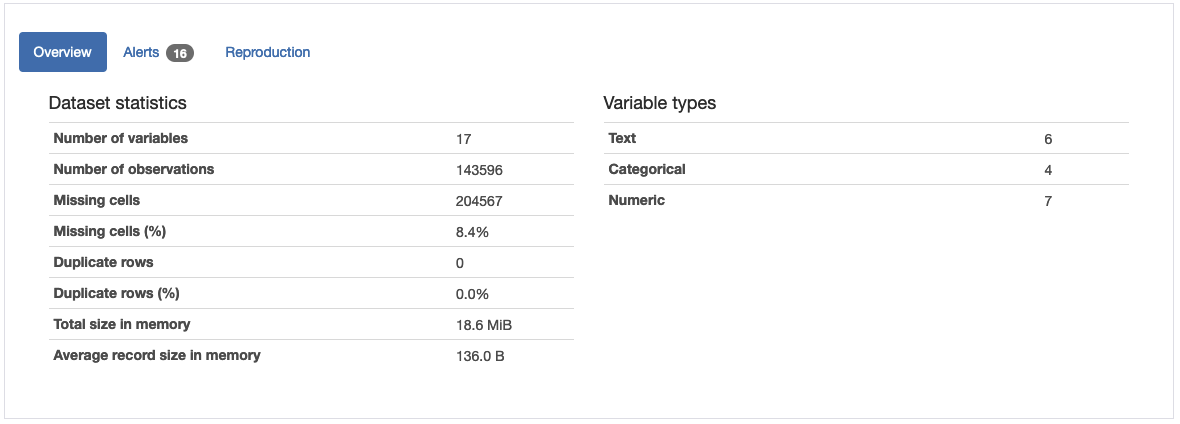
\includegraphics[scale=0.3]{wa_ev.png}
    \caption{WA State EV Data Overview}
    \label{fig:wa_ev}
\end{figure}

\subsubsection{Alternative Fuel Stations By State}
The Alternative Fuel Station data contains 66259 records with the fields
described below (irrelevant fields omitted).  A screenshot of
the overview of the data is provided in Figure \ref{fig:stations}.
\begin{description}
    \item[Station Name] the name of the station;
    \item[Location] the location of the charging station by:
    \begin{itemize}
        \item street address,
        \item city,
        \item state,
        \item postal code,
        \item latitude, and
        \item longitude;
    \end{itemize}
    \item[EVSE Num] the number of charging outlets by type:
    \begin{itemize}
        \item Level 1,
        \item Level 2, and
        \item DC Fast;
    \end{itemize}
    \item[EV Network] the charging network that the station belongs to; and
    \item[Open Date] when the station opened.
\end{description}

\begin{figure}[ht]
    \centering
    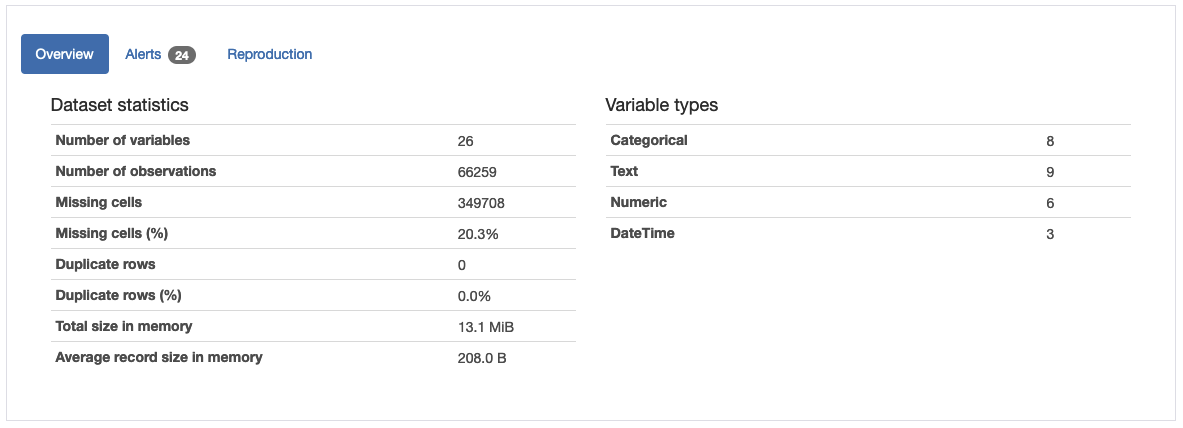
\includegraphics[scale=0.3]{stations.png}
    \caption{Charging Station Data Overview}
    \label{fig:stations}
\end{figure}

Although we initially planned on using vehicle population for the entire US, we
finally decided to abandon that effort for two reasons:
\begin{enumerate}
    \item the sheer size of the dataset (over 5 Gb) would require compute
    resources that we did not have; and
    \item the integration of the datasets was requiring many lookups and
    conversions that were rate-limited (geoid, county, and/or zip-code
    conversions, etc).
\end{enumerate}
Each state provided data in formats that were not standardized with each other,
and location data was stored in ways that made data integration near impossible with
the time frame that we had.  One example of this was where registration data for
vehicles was being stored as congressional districts and/or county name.
Although we found a free API capable of making these conversions, the request
rates are throttled to one request per second.  With this conversion model, we
could make only 86400 requests per day, so with over 1 million records, this
was not viable.

%%%%%%%%%%%%%%%%%%%%%%%%%%%%%%%%%%%%%%%%%%%%%%%%%%%%
% SYSTEM DESCRIPTION
%%%%%%%%%%%%%%%%%%%%%%%%%%%%%%%%%%%%%%%%%%%%%%%%%%%%
\subsection{System Description}

% System Description Here


%%%%%%%%%%%%%%%%%%%%%%%%%%%%%%%%%%%%%%%%%%%%%%%%%%%%
% SCREENSHOTS
%%%%%%%%%%%%%%%%%%%%%%%%%%%%%%%%%%%%%%%%%%%%%%%%%%%%
\subsection{Screenshots}

% System Description Here


\section{Demo Video}
\href{
    % DEMO VIDEO LINK HERE
}{Demo Video}

\section{Project Source Code}
\href{https://github.com/mk-imagine/csc805g5}{EV data visualization project
source code}\\

\end{document}